\documentclass[12pt]{report}

\usepackage[utf8]{inputenc}  % un package
\usepackage[T1]{fontenc}      % un second package
\usepackage[english,french]{babel}
\usepackage{tabularx,ragged2e,booktabs,caption}
\usepackage{multicol} 
\usepackage{color}
\usepackage{amsmath,amssymb,latexsym} 
\usepackage[top=2cm, bottom=3cm, left=2cm, right=2cm]{geometry}
\usepackage{graphicx}
\usepackage{titlesec}
\usepackage{soul}
\setcounter{secnumdepth}{4}
\titleformat{\paragraph}
{\normalfont\normalsize\bfseries}{\theparagraph}{1em}{}
\titlespacing*{\paragraph}
{0pt}{3.25ex plus 1ex minus .2ex}{1.5ex plus .2ex}

\setlength{\parindent}{0pt}
\newcommand{\HRule}{\rule{\linewidth}{0.5mm}}

% \theoremstyle{theorem}
\newtheorem{theorem}{Theorem}[section]
\newtheorem{lemma}[theorem]{Lemma}
\newtheorem{proposition}[theorem]{Proposition}
\newtheorem{corollary}[theorem]{Corollary}
\newtheorem{point}[theorem]{}
\newtheorem{assumption}[theorem]{Assumption}


\theoremstyle{definition}
\newtheorem{definition}[theorem]{Definition}
\newtheorem{example}[theorem]{Example}
\newtheorem{notation}[theorem]{Notation}
\newtheorem{remark}[theorem]{Remark}
\newtheorem{condition}{Condition}

\newcommand{\F}{\operatorname{\mathcal{F}}}
\newcommand{\iF}{\operatorname{\mathcal{F}^{-1}}}

\newcommand{\Loperator}{\mathcal{L}}
%\newcommand{\R}{\mathbf{R}}
\newcommand{\Z}{\mathbf{Z}}

\newcommand{\dd}{\, \textrm{d}}
\newcommand{\e}{\textrm{exp}}
\newcommand{\fFrequency}{ f_{\omega_0}}
\newcommand{\fQuadrature}{ f_{\Delta}}

\newcommand{\I}{\mathbf{I}}

\newcommand{\ErrorFrequency}{\mathcal{E_F}}
\newcommand{\ErrorQuadrature}{\mathcal{E_Q}}
\newcommand{\Error}{\mathcal{E}}
\newcommand{\EF}{\ErrorFrequency}
\newcommand{\EQ}{\ErrorQuadrature}
\newcommand{\est}{\overline {\mathcal{E}}}
\newcommand{\estFrequency}{\est_F}
\newcommand{\estQuadrature}{\est_Q}


\newcommand{\lx}{\mathcal{L}^{X}}
\newcommand{\ls}{\mathcal{L}^{S}}
\newcommand{\R}{\mathbb{R}}
\newcommand{\C}{\mathbb{C}}
\newcommand{\prob}[2]{\pi_{{#1,#2}}}
\newcommand{\lam}[1]{\lambda_#1}
\newcommand{\trials}[2]{\theta_{#1,#2}}
\newcommand{\damp}{\alpha}

\newcommand{\cgmyY}{Y}
\newcommand{\cgmyM}{\eta_+}
\newcommand{\cgmyG}{\eta_-}
\newcommand{\cgmyC}{K}

\newcommand{\cgmyexp}{\cgmyY}

\newcommand{\fa}{f_{\damp}}
\newcommand{\fadisc}[1]{f_{\damp, #1}}
\newcommand{\fdisc}[1]{f_{#1}}
\newcommand{\ga}{g_{\damp}}
\newcommand{\ha}{h_{\damp}}
\newcommand{\ft}[1]{\hat{#1}}
\newcommand{\ift}[1]{\iF\left[#1\right]}
\newcommand{\Lnorm}{\textrm{L}}
\newcommand{\real}[1]{\mathrm{Re}\left[#1\right]}
\newcommand{\im}[1]{\mathrm{Im}\left[#1\right]}
\newcommand{\step}{\Delta\omega}
\newcommand{\strip}[1]{A_{#1}}
\newcommand{\pureJumpProcessConstant}{C(\nu)}

\newcommand{\charExp}[1]{\Psi \parent{{#1}}}
\newcommand{\charFun}[2]{\varphi_{#1} \parent{{#2}}}

\newcommand{\cutoff}{\omega_{\mathrm{\max}}}

\newcommand{\pprob}[1]{}

\newcommand{\fnka}{f_{\damp}^{N,\cutoff}}
\newcommand{\ftnka}{\tilde f_{\damp}^{N,\cutoff}}

\newcommand{\pnka}{\Pi_{\damp}^{N,\cutoff}}

\newcommand{\fft}[2]{\mathrm{FFT}_{{#1}} \parent{{#2} }}
\newcommand{\tol}{\epsilon_{\mathrm T}}

\newcommand{\cutoffFrequency}{\omega_{\textrm{max}}}

\newcommand{\uremark}[2]{\underbrace{{#1}}_{{#2}}}

% Juho macros
\newcommand{\partder}[2]{\frac{\partial #1}{\partial #2}}
\newcommand{\der}[1]{\partial_{ #1}}
\newcommand{\ket}[1]{\left | {#1} \right \rangle }
\newcommand{\refstate}[0]{\textbf{0}}
\newcommand{\vacket}[0]{\ket{\refstate}}
\newcommand{\vacbra}[0]{\bra{\refstate}}
\newcommand{\bra}[1]{\left \langle {#1} \right | }
\newcommand{\ketbra}[1]{\ket{#1} \bra{#1}}
\newcommand{\innerprod}[2]{\left \langle {{#1} | {#2}} \right \rangle}
\newcommand{\uket}[0]{\ket{\uparrow}}
\newcommand{\dket}[0]{\ket{\downarrow}}
\newcommand{\ubra}[0]{\bra{\uparrow}}
\newcommand{\dbra}[0]{\bra{\downarrow}}
\newcommand{\hadj}[1]{{#1}^{\dagger}}
\newcommand{\conj}[1]{{#1}^{\ast}}
\newcommand{\cosine}[1]{\mathrm{cos}\left ( {#1}\right )}
\newcommand{\sine}[1]{\mathrm{sin}\left ( {#1}\right )}
\newcommand{\cosinep}[2]{\mathrm{cos}^{#2}\left ( {#1}\right )}
\newcommand{\sinep}[2]{\mathrm{sin}^{#2}\left ( {#1}\right )}
\newcommand{\expf}[1]{\mathrm{exp}\left ( {#1}\right )}
\newcommand{\expfs}[1]{e^{#1}}
\newcommand{\determinant}[1]{\mathrm{det}\left ( {#1}\right )}
\newcommand{\trace}[1]{\mathrm{Tr}\left ( {#1}\right )}
\newcommand{\parent}[1]{\left( {#1} \right)}
\newcommand{\aver}[1]{ \left\langle  {#1}  \right\rangle }
\newcommand{\absval}[1]{\left| {#1} \right|}
\newcommand{\sset}[1]{\left\lbrace {#1} \right\rbrace }
\newcommand{\iden}[1]{\mathbf{1}_{#1}}
\newcommand{\ssum}[2]{\displaystyle\sum\limits_{#1}^{#2}}
\newcommand{\pprod}[2]{\displaystyle\prod\limits_{#1}^{#2}}
\newcommand{\commut}[2]{\left[ {#1} , {#2} \right]}
\newcommand{\acommut}[2]{\left\lbrace  {#1} , {#2} \right\rbrace }
\newcommand{\spann}[1]{\mathrm{span} \parent{{#1}}}
\newcommand{\ttrace}[2]{\mathrm{Tr}_{#1} \parent{#2}}
\newcommand{\logt}[1]{\mathrm{log_2} \parent{{#1}}}
\newcommand{\hilbert}[1]{\mathcal{H}_{{#1}}}
\newcommand{\genus}{g}
\newcommand{\gsfun}[0]{\eta_{GS}}
\newcommand{\vvec}[1]{\textbf{{#1}}}
\newcommand{\kk}[0]{\vvec{k}}
\newcommand{\tsection}[1]{\newpage \section{{#1}}}
\newcommand{\grad}[0]{\nabla}
\newcommand{\divv}[0]{\nabla \dot}
\newcommand{\curl}[0]{\nabla \times}
\newcommand{\vvar}[1]{\mathrm{var} \parent{{#1}}}
\newcommand{\bigo}[1]{\mathcal O \parent{{#1}}}
\newcommand{\smallo}[1]{ o \parent{{#1}}}
\def\d{\textrm{d}}

\newcommand{\cost}[1]{C_{\mathrm{#1}}}

\newcommand{\qt}[0]{\tilde q}
%\newcommand{\e}[1]{\times 10^{#1}}
\newcommand{\supremum}[1]{\mathop{\mathrm{sup}}_{{#1}}}
\newcommand{\nnorm}[2]{\absval{\absval{{#1}}}_{#2}}
\newcommand{\problem}[1]{\newpage \section*{{#1}}}
\newcommand{\hittime}[0]{\sigma_{\bar{\mathcal E}}}
\newcommand{\probb}[1]{\mathrm{P} \parent{{#1}}}
\newcommand{\expp}[1]{\mathrm{E} \parent{{#1}}}

\newcommand{\kaustaddress}[0]{King Abdullah University of Science and Technology, Thuwal, Kingdom of Saudi Arabia}
\newcommand{\indicatorfun}[3]{\mathbf{1}_{[{#1},{#2}]} \parent{{#3}}}
\newcommand{\indicator}{\mathbf{1}}
\newcommand{\binaryg}[1]{g_{\mathrm{bin}} \parent{#1}}
\newcommand{\binaryf}[1]{f_{\mathrm{bin}} \parent{#1}}
\newcommand{\fbinaryf}[1]{\hat{f}_{\mathrm{bin}} \parent{#1}}

\newcommand{\callg}[1]{g_{\mathrm{call}} \parent{#1}}
\newcommand{\fcallg}[1]{\hat{g}_{\mathrm{call}} \parent{#1}}
\newcommand{\fcallga}[1]{\hat{g}_{\mathrm{call}, \damp} \parent{#1}}
\newcommand{\fputga}[1]{\hat{g}_{\mathrm{put}, \damp} \parent{#1}}
\newcommand{\fcallf}[1]{\hat{f}_{\mathrm{call}} \parent{#1}}
\newcommand{\fcallfa}[1]{\hat{f}_{\mathrm{call}, \damp} \parent{#1}}


\newcommand{\evaldiff}[3]{{\left [ {#1} \right ]}_{#2}^{#3}} 

\newcommand{\vga}{a}
\newcommand{\vgb}{b}

\newcommand{\vgpoly}[1]{w  \parent{#1}}
\newcommand{\vgaux}{q}

\newcommand{\imo}{y}
\newcommand{\reo}{x}
\newcommand{\abex}{\rho}

%%% for the merton case
\newcommand{\sj}{\sigma_{\mathrm{jump}}}
\newcommand{\rj}{r_{\mathrm{jump}}}


%% I always forget the correct spelling
\newcommand{\levy}{L\'evy }
\newcommand{\levynospace}{L\'evy}
%%

\newcommand{\rz}{\R - \sset{0}}

\newcommand{\linf}[1]{L^\infty_{#1}}
\newcommand{\norminf}[2]{\left\|#1\right\|_{\linf{#2}}}


\begin{document}


% This part concern the cover page of the report 
\begin{titlepage}
\begin{center}
\textsc{\Large Tunisia Podfsdaflytechnic School of Tunisia}\\[1.5cm]
\textsc{\Large Graduation project}\\[0.5cm]
% Title
\HRule \\[0.4cm]
{ \huge \bfseries Fourier Transform Methods for Option Pricing \\[0.4cm] }

\HRule \\[1.5cm]

% Author and supervisor
\noindent
\begin{minipage}[t]{0.4\textwidth}
\begin{flushleft} \large
\emph{Author:}\\
Soumaya \textsc{Elkantassi}
\end{flushleft}
\end{minipage}%
\begin{minipage}[t]{0.6\textwidth}
\begin{flushright} \large
\emph{Supervisor:} \\
Prof.~Raul \textsc{Tempone}\\
Fabian\textsc{~Crocce flores}\\
Juho H$\ddot{a}$pp$\ddot{o}$
l$\ddot{a}
$
\end{flushright}
\end{minipage}
\vfill
% Bottom of the page
{\large \today}
\end{center}
\end{titlepage}



\part{Introduction}
\chapter{Black-Scholes-Merton model and its limitations}
\section{Black -Scholes-Merton model}
The Black-Scholes-Merton (or Black and Scholes ) model for evaluating the premium of an option was introduced in 1973 by three economists – Fischer Black, Myron Scholes and Robert Merton. \jcor{}{reference?} They developed a formula to calculate the theoretical \jcor{}{what do you mean by theoretical?} price of European put and call options. This model has become the world's most well-known options pricing formula and has had a significant influence on the way options was traded and priced.\\
\jcor{}{At this point, the whole concept of an option has not been introduced}

Black-Scholes-Merton model assumes that the price, $S$, of an asset follows a geometric Brownian motion,
% equation non centrée
\begin{gather}
dSt = \mu Stdt +\sigma StdWt
\end{gather}

where $\mu$ and $\sigma$ are known constants, 
denoting respectively the expected return and the volatility of the asset and \jcor{$Wt$}{$W_t$} is a standard Brownian motion with drift.\\
\jcom{At this stage, the brownian motion, whether standard or non-standard has not been developed, nor introduced to the reader,
and no mention of the explanation that will follow is made}


Before considering the Black-Scholes option price it is  important to understand the Brownian motion process that has been widely used to determine the return distributions
of assets. The Brownian motion is a particular type of \jcor{Markov}{Markovian} stochastic process, where only the present value of a variable is \jcor{the}{} relevant for prediction the future.\\
Consider a variable, $W_{t_{t \geqslant 0}}$,  following a Brownian motion, then it has the following two properties :\\

$1)$ The change $\Delta W_t$ in a small \jcom{why does this need to be small?} period of time $\Delta t$ is : 
\begin{gather}
\Delta W_t= \sqrt{\Delta t}~ N(0,1)
\end{gather}
\jcom{what is $N(0,1)$}
$2)$ The values of $\Delta W_t$ of any two different short intervals of time,$\Delta t$, are independent(Markov property).
\jcom{this is only true for disjoint intervals, furthermore, I don't see how the independent increments imply markovianness}
 
If we consider the change of $W_t$ in a relatively long period, it can be regarded as the sum of the changes of $\Delta W_t$ in small time intervals of length $\Delta t$:
 \begin{gather}
W(T)-W(0)= \sum\limits_{i=1}^n \sqrt{\Delta t}~ N_i(0,1)  ,  
 \end{gather}
 \jcom{define the time grid for this notation}
where $N_i$ are normally distributed  $N(0,1)$ and  independent from each other.\\
  It follows that $W(T)-W(0)$ is normally distributed $N(0,n\sqrt{\Delta t})$. Hence, the stock returns, $dS_t/S_t$, are assumed to be normally distributed. Normality assumption is one important hypothesis among others in the Black and Scholes model.\\

The graph below shows the variation of a Brownian motion  process when T=1.
\begin{figure}[h]
\centering
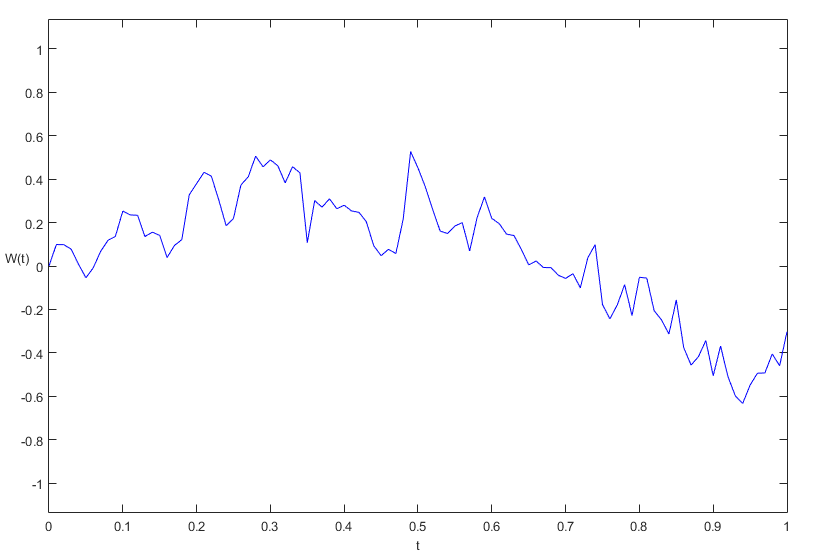
\includegraphics[scale=0.5]{brownian.png} 
\caption{Brownian motion when $\Delta t=0.01$
\jcom{This is a single realisation of a brownian motion. Please include the details of
how this has been computed and the paramters. Furthermore, avoid pixel-rasterized figures.}}
\end{figure} 


To derive the Black-Scholes formula, some assumptions on the assets and the market have been made  :
\begin{itemize}
\item Returns are log-normally distributed.
\item The options are European and can only be exercised at expiration.
\jcor{what is expiration}
\item The stock pays no dividend during the life of the option.
\item The volatility is constant for any strike and maturity.
\item The short-term interest rate (the risk-free rate r) is known and constant through time.
\end{itemize} 


It can be shown that under these assumptions the solution of the stochastic differential equation (1.1) is :
\begin{gather}
St= S_0 e^{\mu-\frac{\sigma^2}{2}+\sigma Wt}
\end{gather}
The Risk Neutral Valuation Theorem \jcom{cite? Under which conditions this theorem holds? When does the
risk neutral probability measure exist?} states that the price of an 
European call $C(St, K,T)$ for any $ t \in [0, T]$, is the discounted expected value of $(S_T-K)^+$ under the risk-neutral probability measure Q .
\begin{gather}
C(St, K,T)= e^{-r \tau} E^Q[(S_t-K)^+|\mathfrak{Ft}] 
\end{gather}
\jcom{Please elaborate on the filtration used!}
Developing this conditional expectation will lead to the following price:
\begin{gather}
C(St,K,T)= S_0 N(d_1) - K e^{-r \tau} N(d_2)
\end{gather}
\jcom{In one way or another girsanov theorem or the like has been employed here?
Where did the dependence on expected returns vanish?}
Where $ d_1= \frac{ln\frac{S_0}{K}+r+\frac{\sigma^2}{2}T}{2} $ and $d_2 = d_1-\sigma \sqrt{T} $ \\
$ S_0$ is the current stock price, T is the time to maturity, $\sigma$ is the stock price volatility,$N(x)$ is the cumulative probability distribution function for the standard normal distribution. The price of the European put option can
be computed by the Put-Call parity. \jcom{derivation, or justification needed}
\begin{gather}
P(St,K,T)= -S_0 N(-d_1) + K e^{-r \tau} N(-d_2)
\end{gather}
\section{Advantages of the Black-Scholes-Merton Model}
\begin{itemize}
\item The expected return $\mu$ does not appear in the Black-Scholes equation. This means the pricing formula is independent of the individual’s preference. 
\jcom{why is this an advantage?}
\item The Black-Scholes equation applies to any derivative asset. \jcom{Is this really true for lookback options, knockdown options and the like?} What distinguishes the different assets are the boundary conditions.
\item The formula (1.4) and (1.5) cancan be easily modified when the interest rate is stochastic or a function of t, when the stock gives dividend or when the
option is American.
\jcom{Can you cite these alterations?}
\item  In the Black-Scholes model, the market operates continuously with the share price following a continuous Ito’s process. \jcom{How is this different from the Brownian motion already mentioned?} This suggests that continuous trading promotes price efficiency and helps investors constantly fine-tune their hedge positions. \jcom{Please define what are hedge positions}
\end{itemize}

These properties together with its simplicity \jcor{makes}{make} the Black-Scholes pricing formula very popular among practitioners for pricing and hedging options. \jcom{How can the formula be used for hedging?}
\section{ Limitations of the Black Scholes Merton Model }
\begin{itemize}
\item \textbf{Non constant volatility}:
Although the Black-Scholes formula is powerful to price stock options, it is widely believed and experimentally verified  that stocks do not have a constant spot volatility, rather this parameter varies with time, e.g. Hull and White(1987), Danilo and Spokoinyi (2004),Goldentyer, Klebaner and Liptser (2005).This may systematically misprice the options and cause the biases of the Black-Scholes model. \jcom{Please add references to these!}


\item \textbf{Non complete market}:
The Black-Scholes-Merton  model assumes that the market is complete,i.e.  that any contingent claim can be perfectly hedged, but if we consider the real situation , the stock price can increase or decrease
lightly like it can fall relatively quickly.So,it is not possible to be hedged against all of these states
simultaneously.The impossibility of perfect hedging means that the market is incomplete\jcor{,}{.} Hence, it makes much more sense to use incomplete market models where the risk of hedging can be quantified rather than sticking to complete market models where the risk of hedging is by definition zero,exponential-Levy models  are examples of incomplete models. \jcom{but black-scholes -model is an exponential levy model!}

\item \textbf{Non Log-normal Distributed returns}: If the stock price follows a geometric Brownian motion with drift  as in equation $(1.1)$, the stock price is log-normally distributed, or, the logarithmic return is normally
distributed.Generally,when dealing with an asset price,this is a poor approximation because, returns often have an excess kurtosis and a non zero skewness values.

\item \textbf{Non continuous process}:
In traditional Brownian diffusion model, price movements are allowed with  small magnitude in short period of time. But in real markets, prices may be have big jumps ,a sudden dramatic decline in short time periods.A good model must be allow for discontinuities and jumps in price process.
\jcom{What exactly is the difference between your description of non-completeness and non-continuousness?}

\end{itemize}

\chapter{Lévy processes and financial modeling}

As seen before \jcom{where?},it is always be more reliable to model prices with a stochastic process involving jumps in order to describe \jcor{the}{} market fluctuations.
Lévy processes, are in fact a valuable tool in financial modeling, because they  provide us with an appropriate
framework that describes adequately real time series.\\


This section \jcor{define}{defines} Lévy processes , \jcor{discuss}{discusses} some of their fundamental properties and \jcor{introduce}{introduces} some examples like Compound \jcor{poison}{Poisson} processes in order to study the use of Lévy models in two categories of financial modeling with \jcor{jums}{jumps} :Jump diffusion and Infinite activity Lévy processes.

\section{ Lévy processes }

A Lévy process is a continuous time stochastic process defined on filtered probability spaces$(\Omega,\mathfrak{I},\mathfrak{I}_{t>0},P)$ ,it has the following properties:\\
\jcom{What are filtered probability spaces}
i)$t \rightarrow X _t$ has cadlag paths, i.e. right-continuous with left limits.\\
ii) $X_0=0$.\\
iii) $X$ has an independent increments, i.e.$ X_t- X_s$ independent from \{ $X_u,{ u \leqslant s}.$\}\\
iv) X has \jcor{stationnary}{stationary} increments $X_t-X_s$ has the same distribution as $ X_{t-s}.$\\
v) X is stochastically continuous,lim $\lim\limits_{k \rightarrow +\infty}$ $P(|X_{t+k}-X_t|  \geqslant \epsilon)=   0 $   $   \forall       \epsilon > 0.$

The fourth property does not imply that the sample paths of $ X_t$ are continuous , it can be regarded as a way to exclude jumps at known time. It means that, at a given time $t$, the \jcor{probabiliy}{probability} of seeing a jump is zero, discontinuities occur just at random times.\\
\jcom{Is this true for an infinite-activity levy process?}

\section{Properties of  Lévy processes :}
\jcom{How exactly are the following properties different in kind from the ones already given?}
$\bullet$ \jcor{Let's}{Let} $(X_t)_{t \geqslant 0}$ be a Lévy \jcor{pocess}{process} on $\mathbb{R}^d$. The every Lévy process can be represented in the following form :
\begin{gather}
X_t= \mu t+ \sigma W_t + \int_0^t \int_{\mathbb{R}/\{0\}} (x-h(x))\nu(x) dx ds 
\end{gather}
where $ W_t $ is continuous geometric \jcom{why geometric?} Brownian motion that can be characterized by two parameters: the drift $\mu$ and the volatility $\sigma$, $\nu(x)$ is a measure on $\mathbb{R}$ called the Lévy measure and  $\int_0^t\int_{\mathbb{R}/\{0\}}(x-h(x))\nu(x) dx ds$ represents the jump part in the process $X_t$. h(x) in an arbitrary truncation function introduced to ensures that the integral part in the Lévy process is integrable.\\
\jcom{}{what is $h$?}


$\bullet$ To count the number of jumps, a Lévy measure is defined via the above formulation :

\begin{gather}
\nu(A)=E[\#\{t \in [0 1]: \Delta X_t \neq 0 , \Delta X_t \in A]
\end{gather}
\jcom{}{Why such definition? Would this not imply an infinite activity for a jumpless model?}
$\nu(A)$ represents the expected number, per unit time, of jumps whose size belongs to $A$.\\
$\bullet$ The distribution of a Lévy process is characterized by its characteristic function, the latter is defined such that :\\
\begin{gather}
\Phi_t(z)=\Phi_{X_t}(z)=E[ e^{izX_t}]
\end{gather}
$\bullet$ There exists a continuous function $\psi $  :$\mathbb{R}^d  \rightarrow \mathbb{R} $, called the characteristic exponent of $X_t$ ,such that:\\
\begin{gather}
E[ e^{izX_t}]= e^ {t \psi (z)}
\end{gather}
\jcom{}{Under which regularity assumptions does this hold true?}
\textbf{ Lévy-Khintchine representation} :\\

$\bullet$ If  $X = (X_t)_{t\geq 0}$  is a Lévy process, then its characteristic function  $\nu_{X_t}(z)$ \jcom{}{This is now the third
notation for a characteristic function, is there a subtlety that I am missing?}  is given by

\begin{equation}
\Phi_t(z)=\mathbb{E}\Big[e^{iz X_t} \Big] =e^ {t \psi (z)}
\end{equation}
\begin{equation}
\psi (z)= \mu iz - \frac{1}{2}\sigma^2  z^2 + 
\int_{\mathbb{R}\backslash\{0\}} \big( e^{izx}-1 -iz h(x)\big)\,\nu(dx) 
\end{equation}

This Lévy–Khintchine representation is fully determined by the Lévy–Khintchine triplet $(\sigma^2,\nu, \mu)$ where $\mu \in $ $\mathbb{R}$ is called the drift term, $\sigma$ the Gaussian or diffusion
coefficient and $\nu$ is the Lévy measure. This triplet is unique for every Lévy process $(X_t)_{t\geq 0}$.\\
$\bullet$ The Lévy measure has no mass at the origin and satisfies the following integrability condition :
\begin{multicols}{2}\noindent
\begin{equation}
 \nu( \{0 \}) = 0
\end{equation}
\begin{equation}
\int_{\mathbb{R}\backslash\{0\}} \big( min \{x^2,1\} ,\nu(dx) < \infty  \Big)
\end{equation}
\end{multicols}

$\bullet$ According to the Lévy Khintchine representation, the characteristic exponent of every Lévy process can be written as the sum of the characteristic exponent of a Brownian motion with drift and the characteristic exponent of a jump component.
$$\psi_B (z)= \mu iz - \frac{1}{2}\sigma^2  z^2 $$
$$\psi_{jump}(z)=\int_{\mathbb{R}\backslash\{0\}} \big( e^{izx}-1 -iz h(x)\big)\,\nu(dx)$$
\jcom{}{Use mathrm for the english subscripts in formulas}

\textbf{Finite/Infinite activity and variation }\\

Considering,$X_t$, a Lévy process with a characteristic triplet $(\sigma^2,\nu, \mu)$ .As we have seen before, the Lévy measure represents the expected number of
jumps of a certain magnitude in a time interval of length 1. Thus, we are able to disguish the class of the Lévy process by reading the lévy measure:
\begin{enumerate}

\item If $\nu$ is a finite
measure,  $\nu(\mathbb{R})= \int_{\mathbb{R}} \nu(dx) < \infty$, then $X_t$ has a finite number of jumps on every finite interval, it is called \emph{finite activity Lévy process}.In this case we dot not need a truncation function $h(x)=0 $.

\item If $\nu$ is an infinite
measure, $\nu(\mathbb{R})=\infty $, an infinite number of jumps \jcor{has}{have} occurred \jcom{Is this intended to be a statement about the individual realisations?}, $X_t$ is then called $\emph{infinite activity Lévy process}$. In this case, conditions $(2.7)$ and $(2.8)$ are no more sufficient to ensure the convergence of the integral part in the Lévy process, some conditions will be imposed on the measure $\nu$ under which we keep the same decomposition of $X_t$ as in $(2.1)$. 

\item if $\sigma = 0$ and $\int_{\mid x\mid
\leqslant1} x\nu(dx) < \infty $, then the path of $X_t$ a has finite variation.
\item if $\sigma \neq 0$ or $\int_{\mid
x\mid
\leqslant
1} x\nu(dx) = \infty $, then the
path of $X_t$ has an infinite variation.
\end{enumerate}
\chapter{ Financial Modeling with Lévy Processes }

After discussing general properties of Lévy processes, we can now give some tractable examples of Lévy processes that can be used in basic financial models and emphasize the different relations between them\jcor{}{.}\\
All the models that will be discussed belong to a family of Lévy processes called “exponential Lévy processes”, under which the dynamic of the underlying stock prices \jcor{is}{are} given by: 
\begin{equation}
S_t= S_0e^{X_t}
\end{equation}
where $X_t$ is a Lévy process under the risk-neutral measure  $\mathbb{Q}$ with
characteristic triplet $(\sigma^2,\nu, \mu)$.
\jcom{}{Isn't the risk-neutral dynamic independent of the expected return?} The log returns log($S_{t}/S_0$) of such a model
\jcor{follows}{follow} the same distribution of the Lévy process $X_t$.
\section{Examples of Lévy process }
\subsection{Poisson process}
The Poisson process counts the number of arrivals in particular time interval.\\
To describe it more clearly, we consider a continuous time arrival process: $ W(u)=\delta(u)$. It is simply an impulse function
\jcom{}{Impulse function is not really a function} every time an event occurs:
\begin{figure}[h]

\centering
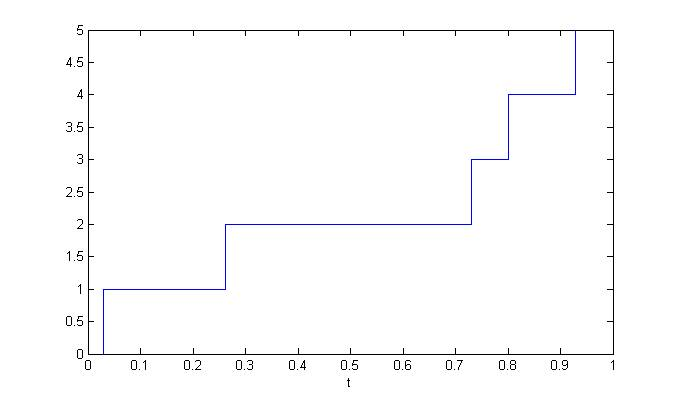
\includegraphics[scale=1]{poisson.jpg} 
\caption{An arrival process in the interval time [0 u]}
\end{figure}
\\
The Poisson process $X_t$ will be the integral of this continuous time arrival process between 0 and t :\\
$X_t=\displaystyle \int_{0}^{t} W(u) \, \mathrm{d}u=\displaystyle \int_{0}^{t} \delta(u) \, \mathrm{d}u$ , which represents the total number of arrivals up to  time t.\\
\jcom{Isn't $\int_{0}^{t} \delta(u) \, \mathrm{d}u=1$ ???}

\begin{figure}[h]

\centering
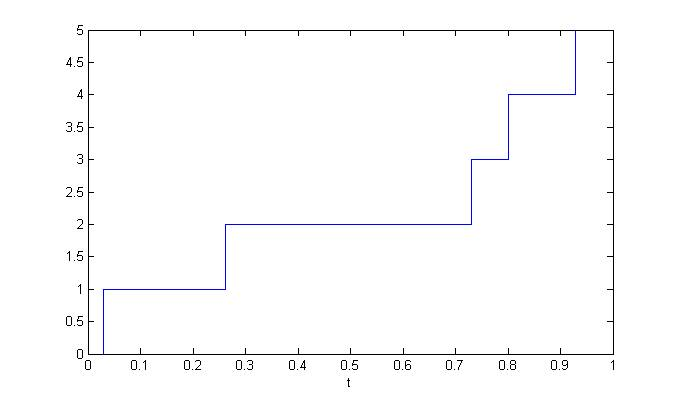
\includegraphics[scale=0.7]{poisson.jpg} 
\caption{Path of Poisson process with intensity $\lambda = 8$}
\end{figure}

As we can see, $X_t$ is continuous time discrete valued process with independent jumps of size one. $X_t$ can be characterized by :\\

i) The waiting time between two successive jumps, it is a random variable called the interarrival time. \\
ii) The interarrival time in the Poisson process follows an exponential distribution that has a very important characteristic called "memorylessness" 
\begin{gather}
 \forall t > s > 0, P(T > t + s|T > t) = P(T > s)
\end{gather}
\jcom{What is the quantity averaged here? Aren't the times deterministic?}

iii) Every Poisson is characterized by a rate parameter $\lambda$, also known as the intensity of the process such that the number of arrivals in time interval $[t, t + \epsilon]$ follows a Poisson distribution with associated parameter \jcor{$\lambda \tau$}{$\lambda \epsilon$} . This relation is given as
\begin{gather}
 P [N(t+ \epsilon) - N(t) = k] = \frac{e^{-\lambda \epsilon} (\lambda \epsilon)^k}{k!}  \qquad k= 0,1,\ldots,
\label{foo}
\end{gather} 
 \jcom{For infinitesimal intervals, $k \geq 2$ is negligible!}
 
\subsection{Compound poisson process}
Let $X_t$ be a Compound Poisson process with intensity $\lambda$ and jump size distribution F, then $X_t$ will be defined as the sum of N(t) jumps arriving randomly according to a Poisson process and having random size specified with the probability distribution F.
\begin{gather}
X(t) = \sum_{i=1}^{N(t)} Y_i
\end{gather}
where,  $\{\,N(t) : t \geq 0\,\}$ is a Poisson process with rate $\lambda$, and $ \{\,Y_i : i \geq 1\,\}$ are independent and identically distributed random variables, with distribution function F.\\
In other words, we could say that a Compound Poisson process is a Poisson process except that the jumps have a random size.

\begin{figure}[h]

\centering
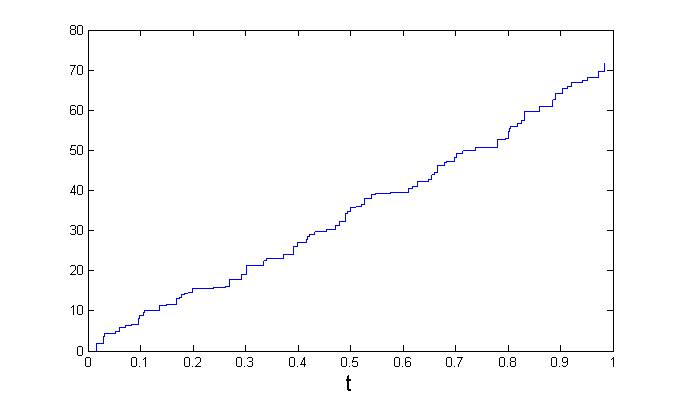
\includegraphics[scale=0.7]{compoisson.jpg} 
\caption{Compound Poisson process with intensity $\lambda=8$
\jcom{How likely is it to have approximately ten times as many jumps as the mean, such as in the picture? Please elaborate on the scheme of simulation you use to produce these plots?}}
\end{figure}
\jcom{What is the distribution of these jumps? Also: how likely is it according to \ref{foo} to have this many jumps? Avoid
pixel rasterisations, when possible. Also, avoid pixel rasterisations like this, there are multiple schemes like tikz and pgfplots that you 
can use to avoid the pixelation of an image.}

\section{Lévy processes in Finance}

Two categories of Lévy processes are used to describe the evolution of market prices. 
The first category is called "Jump-diffusion models": these models have rare jumps and random evolution between the jump times. Such a model can be modeled by a Brownian motion with drift plus a jump part, which is a compound Poisson process .\\

Contrary to Jump-diffusion models, the second category of Lévy processes consists of models with infinite number of jumps in every time interval, called "Infinite activity models".Some of these models could be modeled without Brownian component. Hence, the jump part is the deterministic of the price dynamic, this subcategory is called "infinite activity pure jump models". \jcom{What does it mean that the jump part is the deterministic of something?}
\subsection{Jump diffusion models}
As their name would suggest, these models contain  a diffusion part represented by a Gaussian process (Brownian motion) accentuated by a finite number of jumps(Compound poisson process) with size distribution F.      \\


A Lévy process of jump-diffusion type has the following form: 
\begin{gather}
X_t = \mu t+\sigma W_t+\sum_{i=1}^{N(t)} Y_i
\label{bar}
\end{gather}

where $\mu \in \mathbb{R}, \sigma \in \mathbb{R_+}$, $W_t$ is a standard Brownian motion, $N =(N_t)_{t \geqslant 0}$ is a Poisson process with parameter $\lambda$ (i.e. $E[N_t] = \lambda t$) and $Y = (Y_t)_{t\geqslant 1}$ is an i.i.d. sequence of random variables with probability distribution F. All sources of
randomness $(W_t,N_t,Y_t)$ are mutually independent.

Two famous models of Lévy processes of jump diffusion type are used in modelling the log-price dynamic : The Merton jump-diffusion model and the Kou model.\\

\large\textbf{Merton model}\\


Merton was the first to use a discontinuous price process to model asset returns. (Merton 1976) assumed that the total change in the stock price is posited to be the composition of two types of changes:(1)The ‘normal’ vibrations in price, for example, due to a temporary imbalance between supply and demand, changes in capitalization rates, changes in the economic outlook, or other new information that causes
marginal changes in the stock’s value. In essence, the impact of such information is to produce a marginal change in the price
(almost certainly). This component is modeled by a standard geometric Brownian
motion with a constant variance per unit time and it has a continuous sample
path. (2) The ‘abnormal’ vibrations in price are due to the arrival of important new information about the stock that has more than a marginal effect on price. By its very nature, important information arrives only
at discrete points in time. This component is modeled by a ‘jump’ process reflecting the non-marginal impact of the information.\\


According to the Merton model, the decomposition of the process in given by :
\begin{gather}
X_t = \mu t+\sigma W_t+\sum_{i=1}^{N(t)} Y_i
\label{baz}
\end{gather}
\jcom{How are \ref{bar} and \ref{baz} different?}
where the jump \jcor{size}{sizes} are assumed to have a Gaussian distribution F :
\begin{gather}
F(x) = \frac{1}{\sqrt{2\pi\sigma^2} } e^{ -\frac{(x-\alpha)^2}{2\sigma^2} }
\end{gather}
\jcom{Why constrain to the case in which the jump sizes variance equals the variance of the wiener process?}
Thus, $Y_i  \sim N(\alpha,\sigma^2)$ and the Lévy density :
\begin{gather}
 \nu(x)=\lambda F(x)=\lambda\frac{1}{\sqrt{2\pi\sigma^2} } e^{ -\frac{(x-\alpha)^2}{2\sigma^2} }
\end{gather}
This allows to obtain the probability density of $X_t$ as an expansion series: 
\begin{gather}
p_t(x)=e{-\lambda t} \sum_{k=1}^{\infty} \frac{(\lambda t)^k  e^{ -\frac{(x-\mu t-\alpha k)^2}{2\sigma^2+k \delta^2}}}{k!  \sqrt{2\pi(\sigma^2+k \delta^2)}}
\end{gather}

Taking the parameter values of $S\&P500$ Market from (Andersen and Andreseasen 2001):
\jcom{please include the proper reference}

$ r =5.59 \%,\quad \sigma=17.65\%,\quad  \lambda=8.90\%, \alpha=-88.98\%,\quad  \delta=45.05\%  T=1 year $
\jcom{Why $r$ here and not $\mu$}

we will obtain the following Merton processes. \\


\begin{figure}[h]

\centering
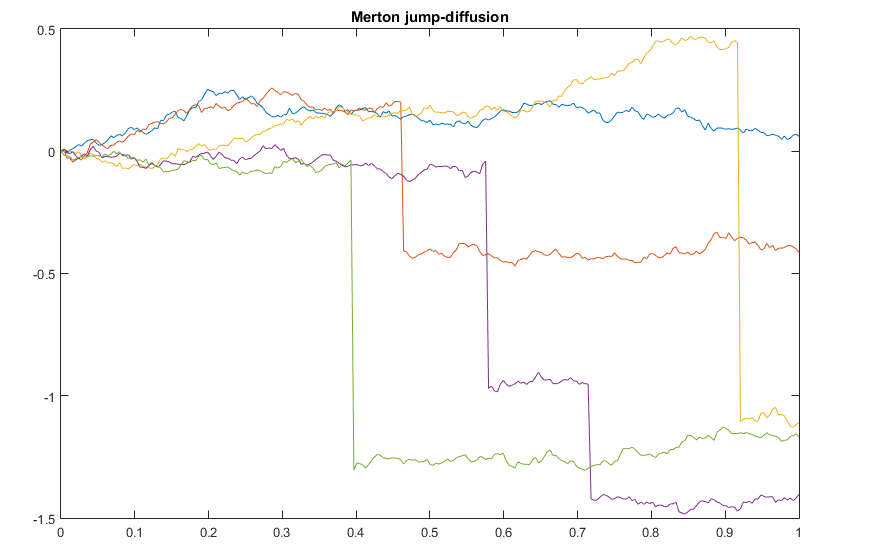
\includegraphics[scale=0.7]{merton.png} 
\caption{Simulated log-price sample paths with Merton model  $\lambda=8$}
\end{figure}
\jcom{Please explain how the simulated realisations have been obtained. Also, how likely is it that one obtains
five independent realisations of a Poisson process with expected number of jumps being 8, such that
all realisations have at most 2 jumps? I assume this probability to be negligible.}
In this graph, the log-price sample path is simulated 5 times in order to see to what extent the source of randomness can change and affect the log-price variation. 
\\


\large\textbf{Kou model}\\

Since the first discontinuous price process proposed by Merton, many researches have been conducted in order to generalize the Black-Scholes model and to incorporate more empirical features(skewness, excess kurtosis and stochastic volatility). This variety of alternative proposed models was presented in Hull (2000) \jcom{citation!}and just like the Black Scholes model they are usually designed to European call and put options.
Hence, it is impossible to derive an analytical solution using these models for other option type such that: American options, lookback options, and barrier options using \jcom{using what} .\\

It was in 2002 that S. G. Kou \jcom{citation!} proposed a jump-diffusion model for option pricing leading to an analytical solution for many option-pricing problems.

Kou demonstrated that double exponential jump size distribution performs well with different option classes  in \jcor{term}{terms} of accuracy and ease of implementation.

The Double Exponential Jump Diffusion Model is given by: 
\begin{gather}
X_t = \mu t+\sigma W_t+\sum_{i=1}^{N^*(t)} Y^*_i
\end{gather}
Where $W_t$ is a standard Brownian motion, $N^* =(N^*_t)_{t \geqslant 0}$ is a Poisson process with parameter $\lambda^*$ (i.e. $E[N_t] = \lambda^* t$) and the log jump sizes $\{Y^*_1 , Y^*_2 , ... \}$ are
independent identically distributed (i.i.d.) random variables such that $Y_i$ has a new double exponential distribution 
\begin{gather}
F(x)= p.\eta_1 \exp \left( -\eta_1 x \right) \mathbf{1}_{\{x\geqslant 0\}}+ q .\eta_2 \exp \left( -\eta_2 x \right) \mathbf{1}_{\{x < 0\}}
\end{gather}
$\lambda > 0,~ \eta_1 > 1, \eta_2 > 0$~,  
$(p,q) \geqslant 0,~ p+q=1$ are the probabilities of the upward and downward jumps of the stock price. So we can
express this also in this way:\\

         \[Y_i = \begin{cases} 
  \zeta^+ ~ with~ a~ probability ~ p \\
         \zeta^-  ~with ~ a ~ probability ~ q
         \end{cases}
          \]
$\zeta^+$ and $\zeta^+$, are exponentially distributed random variables with an expectation value of $\frac{1}{\eta_1}$ and $\frac{1}{\eta_2}$.\\

The lévy measure of the Kou model \jcor{will be defined as below}{is given as}:

\begin{gather}
 \nu(x)=\lambda F(x)=\lambda \big[ p.\eta_1 \exp \left( -\eta_1 x \right) \mathbf{1}_{\{x\geqslant 0\}}+ q .\eta_2 \exp \left( -\eta_2 x \right) \mathbf{1}_{\{x < 0\}}\big]
\end{gather}

Taking the values of Double Exponential Jump Diffusion Model  from (Kou 2002):\jcom{citation!}

$ \eta_1= 10,~\eta_2= 5,~\lambda=1,~\sigma= 16\%,~r=5\%,~ p=0.4,~ q=0.6 ~ and ~T=1 year $\jcom{why need for units for maturity} will lead to the following log-price process.

\begin{figure}[h]

\centering
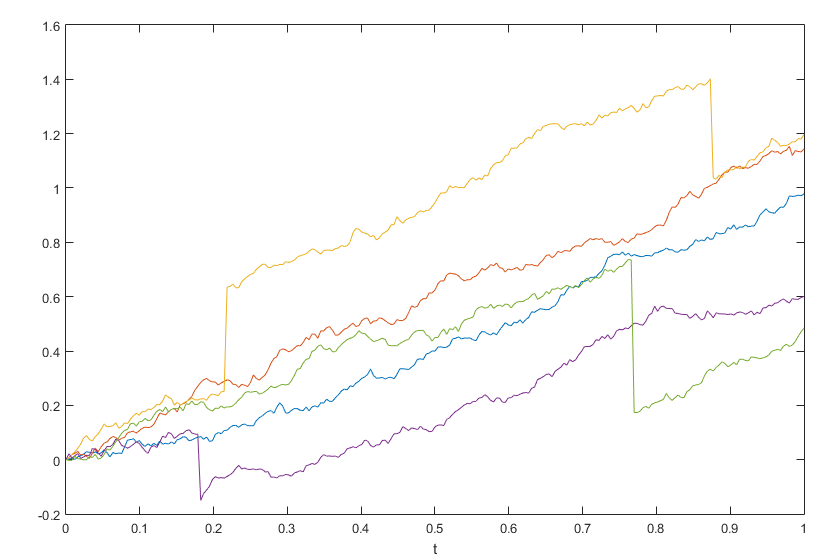
\includegraphics[scale=0.7]{kou.png} 
\caption{Simulated log-price sample paths with Kou model }
\end{figure}
\jcom{Once again, avoid pixel rasterisations. What are the parameters of this plot and how was it generated?}

The values of the parameters \jcor{was}{were} taken from these \jcom{which references?} references in order to be able to benchmark the forward results \jcom{which forward results?} with the exact option price calculated in these papers .

\subsection{Infinite activity pure jump models}

If $\nu$ is an infinite measure, then we are talking about infinite activity Lévy processes. Two conditions should be verified by $\nu$ :\\
- A finite number of large jumps $(|x|>1)$:
$$\int_{|x|>1}|x|\nu( dx)< \infty $$
- Small jumps $(|x|< 1)$ should have finite quadratic variation 

$$\int_{|x|<1}x^2\nu( dx)< \infty $$
In fact,by introducing the truncation function, $h(x)= x\mathbb{I}_{|x|< 1}$ as one of the possible forms \jcom{possible forms of what exactly? I cannot follow the text here?}, in the Lévy process we checked up these two conditions.
\\

\large\textbf{Variance Gamma model}\\

Inside the classes of Lévy processes that allow to build a model for the dynamics of stock prices and have infinite activity, an attention was paid to the Variance Gamma model. This model was proposed by Madan and Seneta(1990) and Carr and Chang(1998) \jcom{citation} and unlike the finite activity models, it can capture the frequent and small jumps as well as infrequent and large ones.\\

The idea of the variance gamma model is to change the time scale of the process by subordinating the Brownian motion to a gamma process. Initially, the variance of the Brownian motion is one, the variance of the changed Brownian motion is gamma distributed, thus, the model is called the \textit{ Variance Gamma  model}. \\   
\jcom{What is $\gamma$ ???}

Consider a traditional Brownian motion:

\[B(t)=B(t,\mu,\sigma)=\mu t +\sigma W(t)\] 

Then, the Variance Gamma model is constructed as below: 
\begin{gather}
 VG(t; \mu,\sigma,\alpha,\beta)=B(\gamma(t,\alpha,\beta);\mu,\sigma) 
\end{gather}


The Lévy measure of the VG model is given by:

 \[\nu_{VG}(y)= \begin{cases} 
  1_{\{y > 0\}} \frac{K e^{y \eta_+}}{y}~ if ~y >0 \\
     1_{\{y < 0\}} \frac{K e^{y \eta_-}}{y}~ if y >0 
         \end{cases}
          \]
\jcom{Why need the indicators if you define the bits with if-clauses. Use mathrm here.}
Taking the following parameter values $\mu= 0.1,\sigma=0.2 \alpha=1 and \beta=1   $, will give us the following log-price simulated paths.
\begin{figure}[h]

\centering
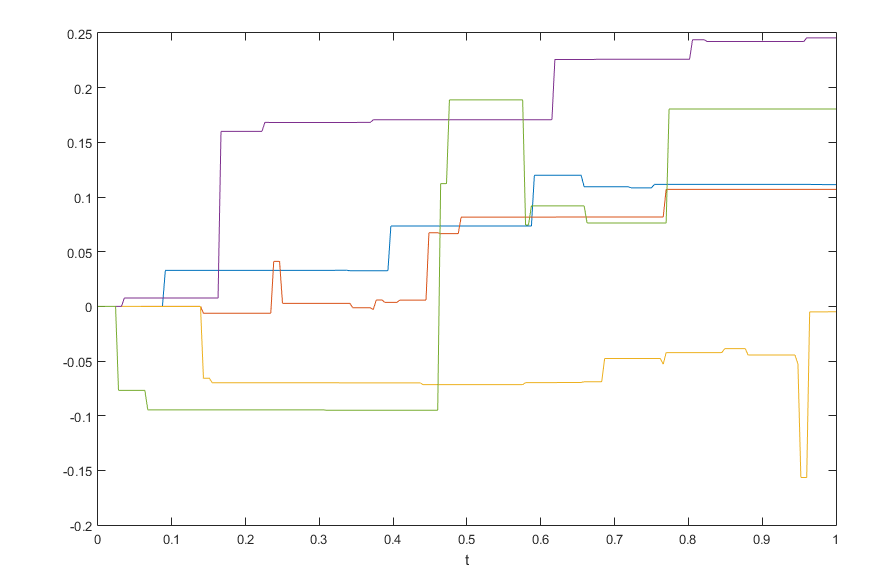
\includegraphics[scale=0.7]{VG.png} 
\caption{Simulated log-price sample paths with Variance Gamma model }
\end{figure}
\jcom{What are the parameters for this model? How was the simulation carried out and why is there only very few jumps?}


\chapter{Fourier Transform Methods For Option pricing }

Various methods can be used to price an option when the underlying
asset price process is modeled by a Lévy process. One can use the famous partial differential equations PDE \jcom{Which ones and under which circumstances is a PDE method sufficient???} and solve it numerically with the finite differences methods which  can be difficult due to the presence of jumps.~Another \jcor{methods}{method} is to use Monte Carlo simulation in order to simulate different paths of the risk neutral process and take the discounted value of the average \jcom{of what} to obtain the option price.~In spite of its efficiency, Monte Carlo simulation is known to be computationally expensive. \jcom{What is meant by this?}\\

There are two reasons why one would choose Fourier transform approach for option pricing:~ 
while the first reason is the unknown probability density of some Lévy processes, the second reason looks more important, since the use of Levy-Khinchine formula allows us not only to recover the analytical expression of the characteristic function but also to work easily in the Fourier space. \jcom{Please elaborate this? What else is achieved than an explicit expression of the characteristic function?}\\

This chapter will introduce Fourier transform approach and demonstrate its effective use for option pricing.~we will also explain the importance of Fast Fourier Transform algorithm FFT in calculating the anti-transform and  \jcor{reduce}{reducing} to overall complexity of the algorithm. 
\newpage
\section{Option price}
Consider an asset whose price at time t is modeled by the stochastic process $S = (St)$
\jcom{please use subscripts in cases like these!!!}
defined by $St = S_0 e^{X_t}$ , where $X = (X_t)$  is assumed to be a Lévy process whose
jump measure is $\nu$.\\
\jcom{Please define what is the risk neutral dynamic. The models thus far make no mention of this!}
Assuming the risk-neutral dynamic for $S_t$, the price at time $t = T-\tau$  of a European option with payoff G and maturity time T is given by


\begin{gather}
\pi(\tau,x)= e^{-r\tau} \expp{G \parent{X_T}|X_{T-\tau} = x}
\end{gather}
where r is the short rate that we assume to be constant and $\tau$ : 0 <$\tau$ < T is the time to
maturity.

\jcom{subscripts!}
Consider $g$ as the reward function in log prices (ie, defined by $g(x) = G(S0ex)$). Now, take f to be defined as
\begin{center}
$f \parent{\tau,x} \equiv \expp{g \parent{X_T}|X_{T-\tau} = x}$
\end{center}

We can observe that f and $ \pi$ are related by :
\begin{gather}
\pi(\tau,S_0 e^x)= e^{-r\tau}f \parent{\tau,x}
\end{gather}
The value of the option $\pi$ is related to the risk-neutral density $p_T$ by:


\jcom{Please elaborate on the homogeneity in log-price-space.}
\begin{align}
\begin{split}
\pi\parent{\tau,x} \equiv & e^{-r\tau}\expp{g \parent{X_T}|X_{T-\tau} = x}
\\
= &e^{-r\tau}\int_\R g\parent{y}  p_\tau \parent{y-x}  \d y
\\
=& e^{-r\tau}\int_\R (S_0 e^y-K)^+ p_\tau \parent{y-x}  \d y, ~~k=log (\frac{K}{S_0})\\
=& e^{-r\tau} \int_k^\infty (S_0 e^y-K) p_\tau \parent{y-x} \d y
\label{moneq}
\end{split}
\end{align}

\jcom{You might want to refer to chapters without explicit numbering to avoid confusion in further edits.}
(See appendix 4.1 for details of the derivation of the discounted expected conditional terminal payoff) 

\section{Fourier Transform approach}

There are different conventions for the Fourier transform. In this section we consider the operator
$\mathbb{F}$ such that

\begin{center}

\jcom{This operator notation is confusing because occasionally the notation you are using is used for describing an abstract field in algebra. I would advise using calligraphic or fractura typeface.}
$\mathbb{F}[f](w)= \int_\R e^{iwx}f(x) dx $
\end{center}
To recover the original function f, we define the inverse Fourier transform as

\begin{center}
$\mathbb{F}^{-1}[\hat{f}] (x) =\frac{1}{2\pi}\int_\R e^{-iwx}f(w) dw $
\end{center}


The principle of the Fourier Transform method is simple: instead of applying the direct discounted expectation, it is easier to compute the integral of its Fourier transform and after that we could recover the option price due to this characteristic:
\begin{center}
$\mathbb{F}^{-1}[\hat{f}] (x)=f(x)$

\end{center} 


From the previous derivation of the option price function eq ~\eqref{moneq}, we could remark that it is not square integrable. To obtain a square integrable function, we would consider a damped version of f defined by $f_{\alpha}(\tau,x) = e^{-\alpha x}f(\tau, x)$.We will discuss later  the choice of $\alpha$.

Now, having an integrable function $f_\alpha$ we can apply the operator $\mathbb{F}$, we will obtain :
\begin{gather}
\hat{f}_{\alpha}(w,\tau)=\int_\R e^{iwx} f_{\alpha}(x,\tau) dx 
\end{gather}


\begin{equation}
f_{\alpha}(x,\tau)=\frac{1}{2\pi}\int_\R e^{-iwx}\hat{f}_{\alpha}(w,\tau) dw
\end{equation}

Thus,\\
\begin{align}
f(x,\tau)= & e^{\alpha x} f_{\alpha}(x,\tau)\\
= & \frac{e^{\alpha x}}{2\pi}\int_\R e^{-iwx}\hat{f}_{\alpha}(w,\tau) dw
\label{souma}
\end{align}

We just have to derive an analytic form for $f_\alpha(w,\tau)$ to put in the equation \eqref{souma} and get back the price of the option.

\begin{align*}
\hat{f}_{\alpha}(w,\tau)= &\int_\R e^{iwx} f_{\alpha}(x,\tau) dx
\\
= &  \int_\R \int_\R \expfs{- \damp x + i \omega x} g \parent{y}  p \parent{y-x} \d y \d \omega
\\
= & \int_\R \int_\R \expfs{ i \omega x} g \parent{y} \expfs{-\damp y} \expfs{-\damp \parent{y
-x}}  p \parent{y-x} \d y \d \omega
\\
= &\hat \ga \parent{\omega} \charFun{\tau}{\omega + i \damp}
\\
= & \hat \ga \parent{\omega} \expfs{\tau \charExp{-i \parent{\omega+i \damp}} }
\\
= & \hat \ga \parent{\omega} \expfs{\tau \charExp{\damp - i \omega} }.
\end{align*}

To obtain the value function we employ the inverse Fourier transformation and
obtain

\begin{equation}
f_{\alpha}(x,\tau)=\frac{1}{2\pi}\int_\R e^{-iwx}\hat{f}_{\alpha}(w,\tau) dw
\end{equation}

or 
\jcom{Use italics only for variables, not (projection) operators.}
\begin{equation}
f_{\alpha}(x,\tau)=\frac{1}{\pi}\int_{0}^{\infty} Re[e^{-iwx}\hat{f}_{\alpha}(w,\tau)] ]dw
\end{equation}


As it is not possible to compute the inverse Fourier transform analytically, we
approximate it by truncating and discretising the integration domain using trapezoidal
quadrature . Consider the following approximation:

\begin{align}
f_{\alpha,\Delta \omega, n}=&\frac{\Delta \omega}{2\pi} \sum \limits_{i=-n}^n e^{-i(k+\frac{1}{2}) \Delta \omega x }\hat{f}_{\alpha}(\omega,\tau)
\\
=& \frac{\Delta \omega}{\pi} \sum \limits_{i=0}^{n-1} Re[e^{-i(k+\frac{1}{2}) \Delta \omega x }\hat{f}_{\alpha}((k+\frac{1}{2}\Delta\omega ),\tau)]
\label{fret}
\end{align}

Thus the option price is: 
\begin{center}

$f_{\Delta \omega, n}(x,\tau)= e^{\alpha x}f_{\alpha,\Delta \omega, n}(x,\tau)$
\end{center}
the discretization formula  error and the complexity 


\section{Fast Fourier Transform Algorithm}
The Fast Fourier Transform algorithm is numerically, efficient method to calculate Discrete Fourier Transform DFT. It was originally developed by Gauss (1805), but not recognized until Cooley and Tukey worked on it(1965).

The DFT is known to approximate a continuous Fourier transform (CFT) to its discrete counterpart:

\begin{equation}
\int_{0}^{\infty} e^{-iwx}f(x) dx ~\approx ~ \sum \limits_{k=0}^{N-1} e^{-i \frac{2\pi}{N}kj} f(x_k)~~~ k=0,...,N-1
\label{FFT}
\end{equation}


If we consider how much complication is involved in this DFT we will find :

- N complex multiplication.



If we consider how much complication is involved in this DFT To get each value of k , we will find :

- N complex multiplication.\\
- N-1 complex additions. 


In total, we have $O(N^2)$ \jcom{What are you trying to say here? You have $N$ complex multiplications and $N-1$ complex additions to evaluate the option price. Then this brings you complexity of $O(N)+O(N)=O(N)$ operations to evaluate the quadrature rule for a single asset value point.} computations for direct DFT. The FFT reduces the complexity from order  $O(N^2)$ to order $O(N log_2N)$.\\
 Although it appears to  have the same computation time, will figure out that FFT makes  a big difference when N is very large.
\begin {table}[h!]
\begin{center}
 \begin{tabular}{||c c c ||} 
 \hline
N & $N^2$ & N $log_2 N$ \\ [0.5ex] 
 \hline\hline
 100 & $10^6$ & $10^4$ \\ 
 \hline
 $10^6$ & $10^{12}$ & $20.10^6$ \\
 \hline
 $10^9$ & $10^{18}$ & $20.10^9$  \\
 \hline

 
\end{tabular}
\jcom{Always include captions to tables and figures and refer to them in the text.}
\title{ DFT vs FFT computation time }

\end{center}
\caption {DFT Vs FFT computation time }
\end{table}


 As we see when N is large the FFT reduces the amount of time that usual DFT takes to perform the option price. we will also see that it provides an efficient way of computing the previous bound eq \eqref{FFT} for several values of x at the same time.\\

 We can clearly notice that the summation in \eqref{fret} is not a direct application of the FFT algorithm. We need to modify it in a way that we obtain 
 
 
 \jcom{I see no bibliography here...}
 
 
 
 
\end{document}